\documentclass{article}

\usepackage[margin=4cm]{geometry}
\usepackage{polyglossia}
	\setmainlanguage{english}
\usepackage{amsmath}
\usepackage{amssymb}
\usepackage{siunitx}
\usepackage{float}
\usepackage{booktabs}
\usepackage{subcaption}
\usepackage{graphicx}
\usepackage{xcolor}
\usepackage{listings}
    \lstset{language=Python,
	basicstyle=\footnotesize\ttfamily,
	breaklines=true,
	framextopmargin=50pt,
	frame=bottomline,
	backgroundcolor=\color{white!85!black},
	commentstyle=\color{blue},
	keywordstyle=\color{red},
	stringstyle=\color{orange!80!black}}
\usepackage{tikz}

\title{Computational Physics - Exercise 9}
\author{Maurice Donner \and Lukas Häffner}

\begin{document}

\maketitle
\newpage

% {{{ Exercise 1
\section{Random Numbers -- Rolling Dice}

We write a simple portable random number generator, using linear congruences:
\begin{align}
    I _{j+1} = a I _{j} + c \ ( \text{mod} \ m )
    \label{LinearCongruence}
\end{align}
For that, we creat an initiation function, that creates a global Variable.

\begin{lstlisting}
def init(initVal):
    global rand
    rand = initVal
\end{lstlisting}

This variable will now be rewritten over and over again by a number generated
by (\ref{LinearCongruence}):

\begin{lstlisting}
def generate_random(a,m,c,initVal):
    global rand
    rand = (a*rand+c)%m
    return rand
\end{lstlisting}

This function produces homogeneously distributed numbers between 0 and m-1.
It can be normalized by \( r_i = I_j /(m-1) \), to get homogeneously distributed
real numbers between 0 and 1. We try it for example for \( a = 106, m = 6075,
c = 1283\):
\begin{lstlisting}
Generating random number... a = 106, m = 6075, c = 1283
Random number sequence:
0: 1389
1: 2717
2: 3760
3: 4968
4: 5441
5: 904
6: 5982
7: 3575
8: 3583
9: 4431

Normalizing...
0: 0.22867961804412248
1: 0.4473164306881791
2: 0.6190319394138953
3: 0.8179124135660191
4: 0.8957853144550544
5: 0.14883108330589398
6: 0.9848534738228515
7: 0.5885742509054989
8: 0.5898913401382944
9: 0.7295027988146197
\end{lstlisting}

A simple way to check 'by eye' that the random number generator really does
produce homogeneously distributed numbers, is to create two sequences with
different initial values \( I_0 \ \text{and} \ J_0 \). 
Let \( \mathbf{r} \) be a random normalized number sequence generated with
\( I_0 = 1 \) and \( \mathbf{s} \) generated with \( J_0 = 2 \).
We plot all pairs \( (r_i, s_i) \) of generated numbers in a number plane:
\begin{figure}[H]
    \centering
    \begin{subfigure}[b]{0.49\linewidth}
	\centering
	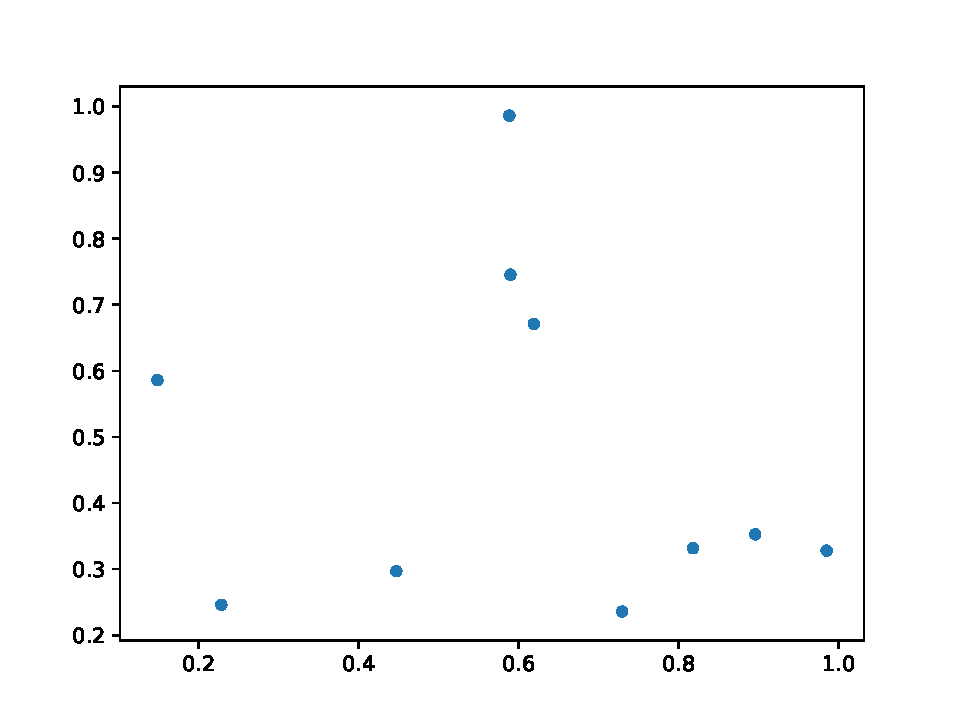
\includegraphics[width=\textwidth]{Fig1-1.pdf} 
	\caption{$n=10$} 
    \end{subfigure}
    \begin{subfigure}[b]{0.49\linewidth}
	\centering
	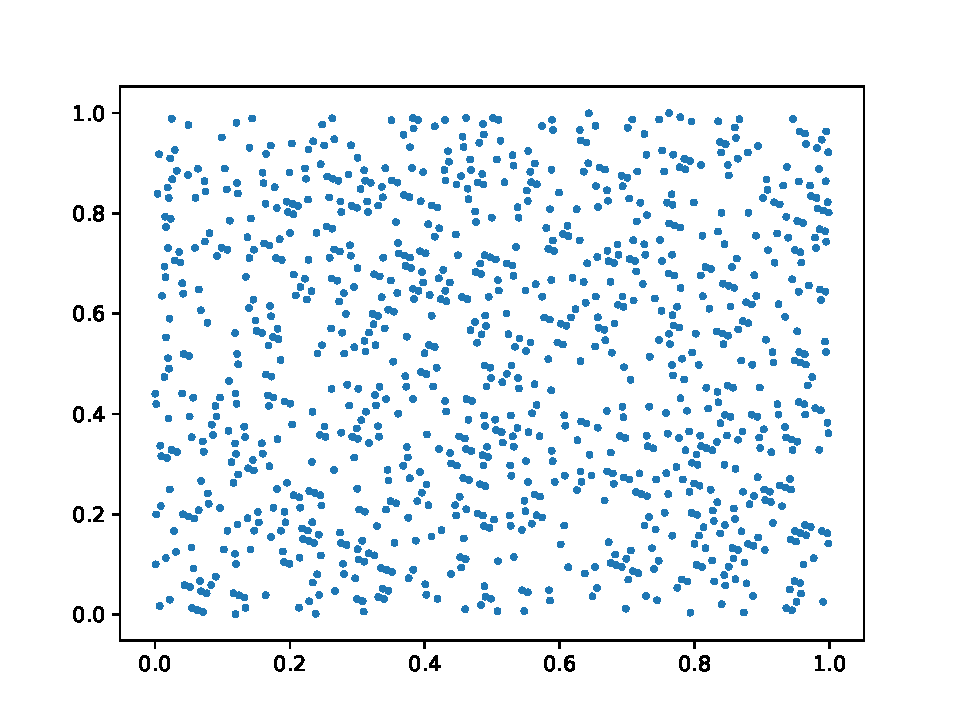
\includegraphics[width=\textwidth]{Fig1-2.pdf} 
	\caption{$n=100$} 
    \end{subfigure}
    \caption{Creating a set of random numbers}
\end{figure}

Since the eye is quite sensitive to see a good distribution, it can safely be
said, that these distributions are indeed what is considered \textit{random}.
To see the deterministic character of this random number sequence, we plot
\( I _{j + 1} \) agains \( I _{j} \) for \( I_0 = 1, \ \text{and} \ n = 100 \):
\begin{figure}[H]
    \centering
    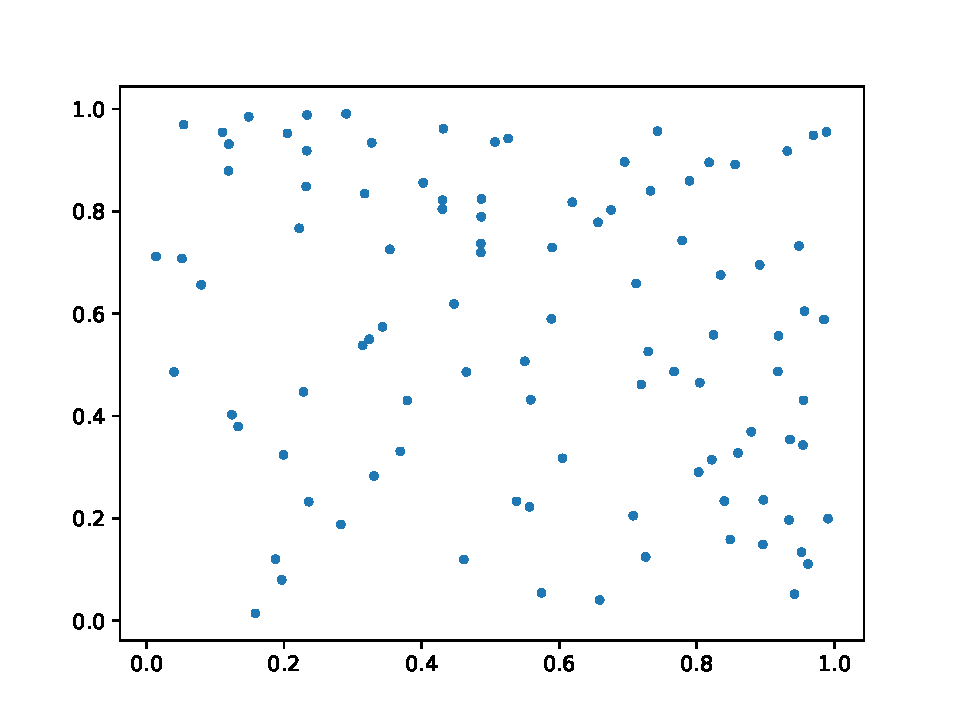
\includegraphics[width=9cm]{Fig1-3.pdf}
    \caption{Deterministic Character of random number sequence}
\end{figure}

% }}}

\end{document}

